%!TEX program = xelatex
\documentclass[10pt, compress, handout]{beamer}
\usepackage[titleprogressbar]{../cls/beamerthemem}

\usepackage{booktabs}
\usepackage[scale=2]{ccicons}
\usepackage{minted}

\usepgfplotslibrary{dateplot}

\usemintedstyle{trac}

\setbeamertemplate{caption}[numbered]
\setbeamertemplate{theorems}[numbered]
\newcounter{example}
\resetcounteronoverlays{example}
\newtheorem{crl}{Corollary}[theorem]
\newtheorem{eg}[example]{Example}
\newtheorem*{solution*}{Solution}

\usepackage{algorithm}
\usepackage[noend]{algpseudocode}

\usepackage{cleveref}
\usepackage{mathtools}
\usepackage{multicol}
\usepackage{qtree}
\usepackage{tikz}

\usepackage{version}
%\excludeversion{proof}
%\excludeversion{solution*}

\makeatletter
\def\old@comma{,}
\catcode`\,=13
\def,{%
    \ifmmode%
    \old@comma\discretionary{}{}{}%
    \else%
    \old@comma%
    \fi%
}
\makeatother

\title{CSCI 3190 Tutorial}
% \subtitle{Assignment 1}
\author{LI Haocheng}
\institute{Department of Computer Science and Engineering}

\begin{document}

\maketitle

\section{Logic and Proofs}
\subsection{Propositional Logic}

\begin{frame}[fragile]
\frametitle{Propositions}
\onslide<1->\begin{eg}
    Which of these sentences are propositions? What are the truth values of those that are propositions?
    \begin{enumerate}
        \item $2 + 3 = 5$.
        \item $5 + 7 = 10$.
        \item $x + 2 = 11$.
        \item Answer this question.
    \end{enumerate}
\end{eg}
\onslide<2>\begin{solution*}
    \begin{enumerate}
        \item Yes, T
        \item Yes, F
        \item No
        \item No
    \end{enumerate}
\end{solution*}
\end{frame}

\begin{frame}[fragile]
\frametitle{Propositions}
\onslide<1->\begin{eg}
    What is the negation of each of these propositions?
    \begin{enumerate}
        \item Sharon has an MP3 player.
        \item There is no pollution in New Jersey.
        \item $2 + 1 = 3$
        \item The summer in HK is hot and sunny.
    \end{enumerate}
\end{eg}
\onslide<2>\begin{solution*}
    \begin{enumerate}
        \item Sharon does not have an MP3 player.
        \item There is pollution in New Jersey.
        \item $2 + 1 \ne 3$
        \item The summer in HK is not
        hot or it is not sunny.
    \end{enumerate}
\end{solution*}
\end{frame}


\begin{frame}[fragile]
    \frametitle{Tautological Implication}
    \onslide<1->\begin{eg}
        Prove the following tautological implication: \begin{equation}
            (p \land (p \rightarrow q) \land (s \lor r) \land (r \rightarrow \lnot q)) \Rightarrow s.
        \end{equation}
    \end{eg}
    \onslide<2>\begin{proof}
        \begin{align}
            \begin{aligned}
            & (p \land (p \rightarrow q) \land (s \lor r) \land (r \rightarrow \lnot q)) \rightarrow s\\
            \equiv & \lnot (p \land (\lnot p \lor q) \land (s \lor r) \land (\lnot r \lor \lnot q)) \lor s\\
            \equiv & \lnot (p \land q \land (\lnot r \lor \lnot q) \land (s \lor r)) \lor s\\
            \equiv & \lnot (p \land q \land \lnot r \land (r \lor s)) \lor s\\
            \equiv & \lnot (p \land q \land \lnot r \land s) \lor s\\ \equiv & \lnot p \lor \lnot q \lor r \lor \lnot s \lor s\\
            \equiv & TRUE.
            \end{aligned}
        \end{align}
    \end{proof}
\end{frame}

\subsection{Propositional Equivalences}

\begin{frame}[fragile]
\frametitle{Logical Equivalence}
\onslide<1->\begin{eg}
    Show that the following are logically equivalent:\begin{enumerate}[(a)]
        \item $\lnot p \land \lnot q \rightarrow \lnot r \equiv r \rightarrow q \lor p$.
        \item $p \rightarrow (q \land r) \equiv (p \rightarrow q) \land (p \rightarrow r)$.
        \item $(p \lor q) \rightarrow r \equiv (p \rightarrow r) \land (q \rightarrow r)$.
        \item $((q \rightarrow p) \land (\lnot p \rightarrow q) \land (q \rightarrow q)) \equiv p$.
    \end{enumerate}
\end{eg}
\onslide<2>\begin{proof}
    \begin{enumerate}[(a)]
        \item $\lnot p \land \lnot q \rightarrow \lnot r \equiv \lnot r \lor \lnot (\lnot p \land \lnot q) \equiv \lnot r \lor (p \lor q) \equiv r \rightarrow q \lor p$.
        \item $p \rightarrow (q \land r) \equiv (q \land r) \lor \lnot p \equiv (\lnot p \lor q) \land (\lnot p \lor r) \equiv (p \rightarrow q) \land (p \rightarrow r)$.
        \item $(p \lor q) \rightarrow r \equiv \lnot (p \lor q) \lor r \equiv (\lnot p \land \lnot q) \lor r    \equiv (\lnot p \lor r) \land (\lnot q \lor r) \equiv (p \rightarrow r) \land (q \rightarrow r)$.
        \item $((q \rightarrow p) \land (\lnot p \rightarrow q) \land (q \rightarrow q)) \equiv ((\lnot q \lor p) \land (p \lor q) \land (\lnot q \lor q)) \equiv ((p \lor (q \land \lnot q)) \land TRUE) \equiv (p \lor FALSE) \equiv p$.
    \end{enumerate}
\end{proof}
\end{frame}

\subsection{Nested Quantifiers}

\begin{frame}[fragile]
\frametitle{Tautology}
\onslide<1->\begin{eg}
    Prove the following statement or find a counterexample to disprove it. All the variables have the
    same domain of the set of all integers:\begin{enumerate}[(a)]
        \item $\forall x \forall y [(x^2 = y^2) \rightarrow (x = y)]$.
        \item $\forall x \exists y [y^2 = x]$.
        \item $\forall x \forall y [xy \ge x]$.
        \item $\exists x \exists y [(x - y = 5) \land (2x + 4y = 4)]$.
    \end{enumerate}
\end{eg}
\onslide<2>\begin{proof}
    \begin{enumerate}[(a)]
        \item False. $x = 1 \land y = -1$ is a counterexample.
        \item False. Let $x = 2$, no integer $y$ satisfying $y^2 = x$.
        \item False. Let $x = 1, y = -1$, we have $xy < x$.
        \item True. Let $x = 4, y = -1$, we have $x - y = 5 \land 2x + 4y = 4$.
    \end{enumerate}
\end{proof}
\end{frame}

\section{Basic Structures}
\subsection{Sets}

\begin{frame}[fragile]
\frametitle{Set}
\begin{columns}
    \begin{column}{.9\linewidth}
        \onslide<1->\begin{eg}
            Determine  whether each of the following statements is true for arbitrary sets $A, B$, and $C$. Give a counterexample if your answer is ``No''.\begin{enumerate}
                \item If $A \in B$ and $B \subseteq C$, then $A \in C$.
                \item If $A \subseteq B$ and $B \in C$, then $A \subseteq C$.
                \item If $A \subseteq B$ and $B \in C$, then $A \in C$.
            \end{enumerate}
        \end{eg}
        \onslide<2>\begin{solution*}
            \begin{enumerate}
                \item Yes.
                \item No. Let $A = \{0\}, B = \{0\}, C = \{\{0\}\}$.
                \item No. Let $A = \emptyset, B = \{0\}, C = \{\{0\}\}$.
            \end{enumerate}
        \end{solution*}
    \end{column}
\end{columns}
\end{frame}

\subsection{Set Operations}

\begin{frame}[fragile]
\frametitle{Set}
\onslide<1->\begin{eg}
    Prove the followings:\begin{enumerate}[(a)]
        \item $A \times (B \cap C) = (A \times B) \cap (A \times C)$.
        \item $(A \cup B) - C = (A - C) \cup (B - C)$.
    \end{enumerate}
\end{eg}
\onslide<2>\begin{proof}
    \begin{enumerate}[(a)]
        \item \begin{align}
        \begin{aligned}
        & ((a, b) \in A \times (B \cap C))\\
        \equiv & ((a \in A) \land (b \in B \cap C))\\
        \equiv & ((a \in A) \land (b \in B) \land (b \in C))\\
        \equiv & (((a, b) \in A \times B) \land ((a, b) \in A \times C))\\
        \equiv & ((a, b) \in (A \times B) \cap (A \times C)).
        \end{aligned}
        \end{align}
        \item $(A \cup B) - C = (A \cup B) \cap \overline{C} = (A \cap \overline{C}) \cup (B \cap \overline{C}) = (A - C) \cup (B - C)$.
    \end{enumerate}
\end{proof}
\end{frame}

\begin{frame}[fragile]
\frametitle{Infinite Set}
\onslide<1->\begin{eg}
    Determine whether the following statements are true or false. \begin{enumerate}[(a)]
        \item If $A$ and $B$ are infinite sets then $A \cap B$ is infinite.
        \item If $B$ is infinite and $A \subseteq B$, then $A$ is infinite.
        \item If $A \subseteq B$ with $B$ finite, then $A$ is finite.
        \item If $A \subseteq B$ with $A$ finite, then $B$ is finite.
    \end{enumerate}
\end{eg}
\onslide<2>\begin{proof}
    \begin{enumerate}[(a)]
        \item False. Let $A = \{x \mid x > 0 \land x \in \mathbb{Z}\}, B = \{x \mid x < 0 \land x \in \mathbb{Z}\}$, then $A \cap B = \emptyset$.
        \item False. Let $B = \mathbb{Z}, A = \emptyset$, then $A \subseteq B, \left|A\right| = 0$.
        \item True. Otherwise, $\left|A\right| > \left|B\right|$ which is contradictory to $A \subseteq B$.
        \item False. Let $A = \emptyset, B = \mathbb{Z}$, then $A \subseteq B, \left|B\right| = \infty$.
    \end{enumerate}
\end{proof}
\end{frame}

\subsection{Functions}

\begin{frame}[fragile]
\frametitle{Function Composition}
\onslide<1->\begin{eg}
    Let $f$, $g$ and $h$ be functions from $\mathbb{N}$ to $\mathbb{N}$, where $\mathbb{N}$ is the set of all natural numbers, i.e., $1, 2, 3, \ldots$
    and are defined as follows: \begin{align}
        f(n) = & 2n + 1,\\
        g(n) = & n + 5,\\
        h(n) = & \begin{cases}
        0 & \text{when $n$ is even},\\
        1 & \text{when $n$ is odd}.
        \end{cases}
    \end{align} Determine $f \circ f, f \circ g, g \circ f$.
\end{eg}
\onslide<2>\begin{solution*}
    \begin{enumerate}[(a)]
        \item $(f \circ f)(n) = 2 (2n + 1) + 1 = 4n + 3$.
        \item $(f \circ g)(n) = 2(n + 5) + 1 = 2n + 11$.
        \item $(g \circ f)(n) = 2n + 1 + 5 = 2n + 6$.
    \end{enumerate}
\end{solution*}
\end{frame}

\begin{frame}[fragile]
\frametitle{Invertible Function}
\onslide<1->\begin{eg}
    If $\left|A\right| = \left|B\right| = 5$, \begin{enumerate}[(a)]
        \item how many function $f: A \rightarrow B$ can be formed?
        \item How many of them are invertible?
    \end{enumerate}
\end{eg}
\onslide<2>\begin{solution*}
    \begin{enumerate}[(a)]
        \item $5^5$.
        \item $5! = 120$.
    \end{enumerate}
\end{solution*}
\end{frame}

\section{Algorithms}
\subsection{Growth of Functions}

\begin{frame}
    \frametitle{Square}
    \begin{columns}
        \begin{column}{0.5\linewidth}
            \onslide<1->\begin{eg}
                Show the following: \begin{enumerate}
                    \item $3n^2 + 5n + 10 = O(n^2)$
                    \item $100 \log_2 n = O(n)$
                    \item $3^n = O(n!)$
                \end{enumerate}
            \end{eg}
            \onslide<2->\begin{proof}
                \begin{enumerate}
                    \item<2-> Let $N = 1, C = 19$, then \begin{equation}
                    \forall n \ge N, 3n^2 + 5n + 10 < C \cdot n^2.
                    \end{equation}
                    \item<3-> Let $N = 4, C = 51$, then $\forall n \ge N, 100 \log_2 n < C \cdot n$.
                    \item<4-> Let $N = 0, C = 5$, then $\forall n \ge N, 3^n < C \cdot n!$.
                \end{enumerate}
            \end{proof}
        \end{column}
        \begin{column}{0.6\linewidth}
            \onslide<1->\begin{eg}
                Determine whether $\log n!$ is $\Theta(n \log n)$.
            \end{eg}
            
            \onslide<5->\begin{proof}
                We can easily show that $(n - i)(i + 1) \ge n$ for $i = 0, 1, \cdots, n - 1$.
                Hence, $(n!)^2 = (n \cdot 1)((n - 1) \cdot 2) \cdot ((n - 2) \cdot 3) \cdots (2 \cdot (n -
                1)) \cdot (1 \cdot n) \ge n^n$. Therefore, $2 log n! \ge n log n$ so that $n \log n$ is $O(\log n!)$.
                
                $\exists c = 1, \exists N = 1$, such that $\forall n \ge N, n! \le n^n$, so that $\log n! \le c n\log n$. Thus $\log n! = O(n \log n)$ so that $n \log n = \Omega(\log n!)$. Hence, $\log n! = \Theta(n \log n)$.
            \end{proof}
        \end{column}
    \end{columns}
\end{frame}

\begin{frame}
    \frametitle{Square Root}
    \begin{columns}
        \begin{column}{0.4\linewidth}
            \onslide<1->\begin{eg}
                Show that $n^2 + 100 \sqrt{n} + 7 = O(n^2)$.
            \end{eg}
            \onslide<2->\begin{proof}
                Let $C = 2, N = 25$, then $\forall n \ge N, n^2 + 100 \sqrt{n} + 7 < Cn^2$.
            \end{proof}
        \end{column}
    \end{columns}
\end{frame}

\section{Induction and Recursion}
\subsection{Mathematical Induction}
\begin{frame}[fragile]
    \frametitle{Division}
    \begin{eg}
        For $n \in \mathbb{N}^+$, prove each of the following by mathematical induction:\begin{enumerate}
            \item $3 | 2^{2n + 1} + 1$;
            \item $9 | n^3 + (n + 1)^3 + (n + 2)^3$.
        \end{enumerate}
    \end{eg}
    \begin{proof}
        \begin{enumerate}
            \item<2-> \begin{description}
                \item[Base] Let $n = 0$, $3 \mid 2^1 + 1 = 3$.
                \item[Induction] Suppose $3 \mid 2^{2n - 1} + 1$, $2^{2n + 1} = 2^{2n - 1} \times 3 + 2^{2n - 1} + 1$
                $\equiv 0 \pmod{3}$.
            \end{description}
            \item<3> \begin{description}
                \item[Base] Let $n = 0$, $9 \mid 1^3 + 2^3$.
                \item[Induction] Suppose $9 \mid (n - 1)^3 + n^3 + (n + 1)^3$, $n^3 + (n + 1)^3 + (n + 2)^3$
                $= (n - 1)^3 + n^3 + (n + 1)^3 + 3((n - 1)^2 + (n - 1)(n + 2) + (n + 2)^2)$
                $= (n - 1)^3 + n^3 + (n + 1)^3 + 9(n^2 + n + 1) \equiv 0 \pmod{9}$.
            \end{description}
        \end{enumerate}
    \end{proof}
\end{frame}

\begin{frame}
    \frametitle{Sequence}
    \begin{columns}
        \begin{column}{0.4\linewidth}
            \onslide<1->\begin{eg}
                Prove by mathematical induction that \begin{equation}
                \sum_{i = 1}^{n} \frac{1}{i^2} < 2 - \frac{1}{n}.
                \end{equation}
            \end{eg}
        \end{column}
        \begin{column}{0.7\linewidth}
            \onslide<3->\begin{proof}
                \begin{description}
                    \item[Basis step] When $n = 2$,
                    it's obvious that $1 + \frac{1}{4} < 2 - \frac{1}{2}$.
                    \item[Inductive step] Let statement $P(n)$ be $\sum_{i = 1}^{n} \frac{1}{i^2} < 2 - \frac{1}{n}$. When $P(k)$ is true, \begin{align}
                    \begin{aligned}
                    \sum_{i = 1}^{k + 1} \frac{1}{i^2} = & \sum_{i = 1}^{k} \frac{1}{i^2} + \frac{1}{(k + 1)^2}\\
                    < & 2 - \frac{1}{k} + \frac{1}{k(k + 1)}\\
                    = & 2 - \frac{1}{k + 1}.
                    \end{aligned}
                    \end{align}
                    Then $P(k + 1)$ is also true.
                \end{description}
            \end{proof}
        \end{column}
    \end{columns}
\end{frame}

\begin{frame}
    \frametitle{Right Triominoes}
    \begin{columns}
        \begin{column}{.3\linewidth}
            \begin{eg}
                Let $n \in \mathbb{N}^+$. Show that every $2^n \times 2^n$ checkerboard with one square removed can be tiled using right triominoes, where these pieces cover three squares at a time.
            \end{eg}
            \begin{figure}
                
\includegraphics[width=.4\linewidth]{triomino}
                \caption{Triomino}
            \end{figure}
        \end{column}
        \begin{column}{.8\linewidth}
            \begin{proof}
                \begin{description}
                    \item[Base]<2-> $P(1)$ is true, obviously.
                    \item[Induction]<3> Split the $2^{k + 1} \times 2^{k + 1}$ checkerboard with one square removed into four checkerboards of size $2^k \times 2^k$. Now temporarily remove the
                    square from each of the three full checkerboards at the center of the original. By the inductive hypothesis,
                    each of these four checkerboards with a square removed can be tiled by right triominoes. Furthermore, the three squares that were temporarily removed can be covered by one right
                    triomino.
                \end{description}
            \end{proof}
        \end{column}
    \end{columns}
\end{frame}

\subsection{Recursive Algorithms}

\begin{frame}
    \frametitle{Exponential}
    \begin{columns}
        \begin{column}{0.6\linewidth}
            \onslide<1->\begin{eg}
                \label{eg:inr:algo:exp}
                Devise a recursive algorithm to compute $a^{2^n}$,
                where $a \in \mathbb{R} \land n \in \mathbb{N}^+$.
            \end{eg}
            \onslide<2->\begin{solution*}
                The complexity of~\Cref{a:inr:algo:exp} is $O(n)$.
                \begin{algorithm}[H]
                    \caption{Recursive Algorithm}
                    \label{a:inr:algo:exp}
                    \begin{algorithmic}
                        \Procedure{Exp}{$n$, $a$}
                        \If{$n$ = 0}
                        \State \Return $a$
                        \Else
                        \State $p \leftarrow$ \Call{Exp}{$n - 1$, $a$}
                        \State \Return $p \times p$
                        \EndIf
                        \EndProcedure
                    \end{algorithmic}
                \end{algorithm}
            \end{solution*}
        \end{column}
        \begin{column}{0.5\linewidth}
            \onslide<1->\begin{eg}
                Repeat~\Cref{eg:inr:algo:exp} with an iterative algorithm.
            \end{eg}
            \onslide<3>\begin{solution*}
                The complexity of~\Cref{a:6-b} is $O(n)$.
                \begin{algorithm}[H]
                    \caption{Iterative Algorithm}
                    \label{a:6-b}
                    \begin{algorithmic}
                        \Procedure{Exp}{$n$, $a$}
                        \For{$i = 1, \ldots, n$}
                        \State $a \leftarrow a \times a$
                        \EndFor
                        \State \Return $a$
                        \EndProcedure
                    \end{algorithmic}
                \end{algorithm}
            \end{solution*}
        \end{column}
    \end{columns}
\end{frame}

\begin{frame}[allowframebreaks]
    \frametitle{Fibonacci}
    \begin{eg}
        Consider the computation of the $n$-th Fibonacci number:\begin{enumerate}
            \item Give the pseudo code of a recursive algorithm to compute the nth Fibonacci number. What is the
            complexity of your algorithm? Explain your answer.
            \item Give the pseudo code of an iterative algorithm to compute the nth Fibonacci number. What is the
            complexity of your algorithm? Explain your answer. 
        \end{enumerate}
    \end{eg}
    
    \newpage
    
    \begin{solution*}
        \begin{columns}
            \begin{column}{.6\linewidth}
                \begin{algorithm}[H]
                    \caption{Recursive Algorithm}
                    \label{a-4-1}
                    \begin{algorithmic}
                        \Procedure{Fib}{$n$}
                        \If{$n = 0$}
                        \State\Return $0$
                        \EndIf
                        \If{$n = 1$}
                        \State\Return $1$
                        \EndIf
                        \State\Return \Call{Fib}{$n - 1$} + \Call{Fib}{$n - 2$}
                        \EndProcedure
                    \end{algorithmic}
                \end{algorithm}
                
                $O(a_n) = \left(\frac{\sqrt{5} + 1}{2}\right)^n$.
            \end{column}
            
            \begin{column}{.5\linewidth}
                \begin{algorithm}[H]
                    \caption{Iterative Algorithm}
                    \label{a-4-2}
                    \begin{algorithmic}
                        \Procedure{IterFib}{$n$}
                        \If{$n = 0$}\ \Return $0$
                        \EndIf
                        \State $x \coloneqq 0, y \coloneqq 1$
                        \For{$i \coloneqq 1, 2, \cdots, n - 1$}
                        \State $z \coloneqq x + y, x \coloneqq y, y \coloneqq z$
                        \EndFor
                        \State \Return $y$
                        \EndProcedure
                    \end{algorithmic}
                \end{algorithm}
                
                The number of additions follows the expression $b_n = n - 1$ so that $O(b_n) = n$.
            \end{column}
        \end{columns}
    \end{solution*}
\end{frame}

\begin{frame}
    \frametitle{Mode}
    \begin{columns}
        \begin{column}{0.4\linewidth}
            \onslide<1->\begin{eg}
                Give a recursive algorithm for finding the sum of the first $n$ positive integers.
            \end{eg}
            \onslide<3->\begin{solution*}
                \begin{algorithm}[H]
                    \caption{A Recursive Algorithm for Summation}
                    \label{a-2}
                    \begin{algorithmic}
                        \Procedure{sum}{$n \in \mathbb{N}$}
                        \If{$n = 0$}
                        \State\Return $0$
                        \EndIf
                        \State\Return $n + $\Call{sum}{$n - 1$}
                        \EndProcedure
                    \end{algorithmic}
                \end{algorithm}
            \end{solution*}
        \end{column}
        \begin{column}{0.7\linewidth}
            \begin{eg}
                Give a recursive algorithm for finding a mode of a list of integers.
            \end{eg}
            \onslide<2>\begin{solution*}
                \begin{algorithm}[H]
                    \caption{A Recursive Algorithm for Mode}
                    \label{algo:inr:algo:mode}
                    \begin{algorithmic}
                        \Procedure{mode}{$a_1, \cdots, a_n \in \mathbb{Z}$}
                        \If{$n = 1$}
                        \Return $a_1$
                        \EndIf
                        \State $m \eqqcolon $ \Call{mode}{$a_1, \cdots, a_{n - 1}$}
                        \If{$m = a_n$}
                        \Return $a_n$
                        \EndIf
                        \State $numM \eqqcolon$ number of $m$ in $a_1, \cdots, a_n$
                        \State $numN \eqqcolon$ number of $a_n$ in $a_1, \cdots, a_n$
                        \If{$numM \le numN$}
                        \Return $a_n$
                        \EndIf
                        \State\Return $m$
                        \EndProcedure
                    \end{algorithmic}
                \end{algorithm}
            \end{solution*}
        \end{column}
    \end{columns}
    
\end{frame}

\begin{frame}[fragile]
    \frametitle{Recursion Algorithm}
    \begin{eg}
        Give a recursive algorithm for tiling a $2^n \times 2^n$ checkerboard with one square missing using right triominoes.
    \end{eg}
    \onslide<2>\begin{solution*}
        If $n = 1$ (basis step), place the one right triomino so that its
        armpit corresponds to the hole in the $2 \times 2$ board. If $n > 1$, then
        divide the board into four boards, each of size $2^{n - 1} \times 2^{n-1}$,
        notice which quarter the hole occurs in, position one right triomino
        at the center of the board with its armpit in the quarter
        where the missing square is, and
        invoke the algorithm recursively four times -- once on each of
        the $2^{n - 1} \times 2^{n - 1}$ boards, each of which has one square missing.
    \end{solution*}
\end{frame}

\begin{frame}[fragile]
    \frametitle{Merge Sort}
    \begin{eg}
        Prove that the merge sort algorithm is correct.
    \end{eg}
    \onslide<2>\begin{proof}
        If
        $n = 1$, then the algorithm does nothing, which is correct because
        a list with one element is already sorted. Assume that
        the algorithm works correctly for $n = 1$ through $n = k$. If
        $n = k + 1$, then the list is split into two lists, $L_1$ and $L_2$. By the
        inductive hypothesis, \textit{mergesort} correctly sorts each of these
        sublists; furthermore, \textit{merge} correctly merges two sorted lists
        into one because with each comparison the smallest element
        in $L_1 \cup L_2$ not yet put into $L$ is put there.
    \end{proof}
\end{frame}

\section{Counting}
\subsection{The Pigeonhole Principle}

\begin{frame}[fragile]
\frametitle{Friends or Enemies}
\begin{eg}
    Assume that in a group of six people, each pair of individuals consists of two friends or two enemies.
    Show that there are either three mutual friends or three mutual enemies in the group.
\end{eg}
\onslide<2>\begin{solution*}
    Let $A$ be one of the six individuals.
    Following from the generalized pigeonhole principle, of the five other people in the group,
    there are either three or more who are friends or enemies of $A$.
    
    Without loss of generality, suppose that $B$, $C$, and $D$ are friends of $A$.
    If any two of these three people are friends,
    then these two and $A$ form a group of three mutual friends.
    Otherwise, $B$, $C$, and $D$ form a set of three mutual enemies.
\end{solution*}
\end{frame}

\begin{frame}
    \frametitle{Adding up to Sixteen}
    \begin{columns}
        \begin{column}{0.6\linewidth}
            \onslide<1->\begin{eg}
                How many numbers must be selected from the set $\{1, 3, 5, 7, 9, 11, 13, 15\}$ to guarantee that at
                least one pair of these numbers add up to 16? Explain your answer using the pigeonhole principle.
            \end{eg}
            \onslide<2->\begin{solution*}
                There are four pairs can add up to 16. Form the set into four pigeonholes accordingly, let the selected numbers be pigeons. At least five pigeons must be selected to guarantee that at least one hole has two pigeons.
            \end{solution*}
        \end{column}
        \begin{column}{0.4\linewidth}
            \onslide<1->\begin{eg}
                What is the least number of comparisons needed to merge any two lists in increasing order into one list in increasing order when the number of elements in the two lists are
                
                A) 1, 4? B) 2, 4? C) 3, 4? D) 4, 4?
            \end{eg}
            \onslide<3>\begin{solution*}
                A.
            \end{solution*}
        \end{column}
    \end{columns}
\end{frame}

\subsection{Permutations and Combinations}
\begin{frame}[fragile]
\frametitle{Permutation}
\begin{columns}
    \begin{column}{.6\linewidth}
        \begin{definition}
            A \textbf{permutation} of a set of distinct objects is an ordered arrangement of these objects.
        \end{definition}
        \begin{definition}
            An ordered arrangement of $r$ elements of a set is called an \textbf{$r$-permutation}.
        \end{definition}
        \begin{theorem}
            \label{thm:p}
            If $n$ is a positive integer and $r$ is an integer with $1 \le r \le n$, then there are $P(n, r) = n(n - 1)(n - 2) \cdots (n - r + 1)$
            $r$-permutations of a set with $n$ distinct elements.
        \end{theorem}
    \end{column}
    \begin{column}{.5\linewidth}
        \onslide<2>\begin{proof}
            The first element of the
            permutation can be chosen in $n$ ways. There are $n - 1$ ways to choose the second element of the permutation. Similarly, there are $n - 2$ ways to choose the third element, and so on, until there are exactly $n - (r - 1) = n - r + 1$ ways to choose the $r$th element. Consequently, by the product rule, there are
            $n(n - 1)(n - 2) \cdots (n - r + 1)$
            $r$-permutations of the set.
        \end{proof}
    \end{column}
\end{columns}
\end{frame}

\begin{frame}[fragile]
\frametitle{Factorial Expression}
\begin{columns}
    \begin{column}{.5\linewidth}
        \onslide<1->\begin{eg}
            How many ways are there to select a first-prize winner, a second-prize winner, and a third-prize winner from 100 different people who have entered a contest?
        \end{eg}
        \onslide<2->\begin{solution*}
            The number is the number of 3-permutations of a set of 100 elements. Consequently, the answer is ${}_{100}P_3 = 100 \times 99 \times 98 = 970200$.
        \end{solution*}
    \end{column}
    \begin{column}{.6\linewidth}
        \onslide<1->\begin{eg}
            How many times does \texttt{plan}, \texttt{than} and \texttt{both} NOT occur in permutations of the 26 letters?
        \end{eg}
        \onslide<3>\begin{solution*}
            \texttt{plan} occurs $23!$ times.
            
            \texttt{than} occurs $23!$ times.
            
            \texttt{both} occurs $23!$ times.
            
            \texttt{plan} and \texttt{than} occurs $0$ times.
            
            \texttt{plan} and \texttt{both} occurs $20!$ times.
            
            \texttt{than} and \texttt{both} occurs $21!$ times.
            
            \texttt{plan}, \texttt{than} and \texttt{both} occurs $0$ times.
            
            So the answer is $26! - 23! \times 3 + 21! + 20!$.
        \end{solution*}
    \end{column}
\end{columns}
\end{frame}

\begin{frame}[fragile]
\frametitle{Onto}
\begin{eg}
    Consider the set $X$ of all functions $f \colon A \rightarrow B$, where $A = \{1, 2, 3, 4, 5, 6, 7\}$, $B = \{a, b, c, d, e\}$. How many functions in $X$ are onto?
\end{eg}
\onslide<2>\begin{solution*}
    For the first situation that 1 of $B$ matches 3 of $A$ and others match 1 of $A$ for each, we select 4 of 5 in $B$ and for each of them select 1 different item in $A$ so that there are ${}_4 C_1 \times {}_7 P_4$ functions in the first situation.
    
    For the second situation that 2 of $B$ match 2 of $A$ for each and others match 1 of $A$ for each, we select 3 of 5 in $B$, for each of them select 1 different item in $A$ and then from the rest 4 items in $A$ select 2 of them to match 1 of 2 rest item in $B$ so that there are ${}_5 C_2 \times {}_7 P_3 \times {}_4 C_2$ functions in the section situation.
    
    Totally, there are ${}_5 C_1 \times {}_7 P_4 + {}_5 C_2 \times {}_7 P_3 \times {}_4 C_2 = 16800$ functions.
\end{solution*}
\end{frame}

\section{Advanced Counting Techniques}
\subsection{Applications of Recurrence Relations}

\begin{frame}[fragile]
\frametitle{Codeword Enumeration}
\begin{eg}
    \label{eg:8}
    Computer system considers a string of decimal digits a valid
    codeword if it contains an even number of 0 digits. For instance, 1230407869 is valid,
    whereas 120987045608 is not valid. Let $a_n$ be the number of valid $n$-digit codewords. Find
    a recurrence relation for $a_n$.
\end{eg}

\onslide<2>\begin{solution*}
    There are nine 1-digit codewords so that $a_1 = 9$.
    There are two ways to form
    a valid string with $n$ digits from a string with one fewer digit.
    First, it can be obtained by appending a valid string of $n - 1$ digits with a digit other than 0, which has $9a_{n - 1}$ ways.
    Second, it can be obtained by appending a 0 to a string of length $n - 1$ that is not valid, which has $10_{n - 1} - a_{n - 1}$ ways.
    Because all valid strings of length n are produced in one of these two ways, it follows that there are $a_n = 9 a_{n - 1} + (10^{n - 1} - a_{n - 1}) = 8 a_{n - 1} + 10^{n - 1}$ valid strings of length $n$.
\end{solution*}
\end{frame}

\begin{frame}[allowframebreaks]
    \frametitle{Double Tower of Hanoi}
    \begin{eg}
        A Double Tower of Hanoi contains $2n$ disks of $n$ different sizes, two of each size. As usual, we can move
        only one disk at a time, without putting a larger one over a smaller one. Assume that disks of equal size are
        indistinguishable from each other:\begin{enumerate}[(a)]
            \item Write a pseudo-code to solve the above problem recursively.
            \item Set up a recurrence equation to count the number of steps to move $2n$ disks. 
            \item Solve the recurrence equation and give the complexity of your algorithm.
        \end{enumerate}
    \end{eg}
    \begin{solution*}
        \begin{columns}
            \begin{column}{.5\linewidth}
                \begin{enumerate}[(a)]
                    \item See Algorithm \ref{a-3}.
                    \item $H_{2n} = 2H_{2n - 2} + 2$.
                    \item \begin{align}
                    H_{2n} & = 2(2H_{2n - 4} + 2) + 2\\
                    & = 4H_{2n - 4} + 4 + 2\\
                    & \cdots\\
                    & = 2^{n + 1} - 2.\\
                    & = O(2^n).
                    \end{align}
                \end{enumerate}
            \end{column}
            \begin{column}{.5\linewidth}
                \begin{algorithm}[H]
                    \caption{Double Tower of Hanoi}
                    \label{a-3}
                    \begin{algorithmic}
                        \Procedure{Hanoi}{$h$, $b$, $e$, $m$}
                        \If{$h$ = 0}
                        \State \Return
                        \ElsIf{$h$ = 2}
                        \State \Call{Move}{$b$, $e$}
                        \State \Call{Move}{$b$, $e$}
                        \Else
                        \State \Call{Hanoi}{$h - 2$, $b$, $m$, $e$}
                        \State \Call{Hanoi}{2, $b$, $e$}
                        \State \Call{Hanoi}{$h - 2$, $m$, $e$, $b$}
                        \EndIf
                        \EndProcedure
                    \end{algorithmic}
                \end{algorithm}
            \end{column}
        \end{columns}
    \end{solution*}
\end{frame}

\begin{frame}
    \frametitle{Hanoi Tower}
    \begin{columns}
        \begin{column}{0.6\linewidth}
            \onslide<1->\begin{eg}
                Consider the Tower of Hanoi problem with peg A, B, C. We want to transfer a tower of $n$ disks
                from A to B, if direct moves between A and B are disallowed. \begin{enumerate}
                    \item Write a recursive pseudocode.
                    \item Set up a recurrence equation to count the number of steps to move $n$ disks.
                \end{enumerate}
            \end{eg}
            \begin{solution*}
                \begin{enumerate}
                    \item<2-> See~\Cref{a:5-1}.
                    \item<3> Let the number of steps to move $n$ disks be $\{s_n\}$, then $s_0 = 0, s_n = 3s_{n - 1} + 2$.
                \end{enumerate}
            \end{solution*}
        \end{column}
        \begin{column}{0.5\linewidth}
            \onslide<2->\begin{algorithm}[H]
                \caption{Tower of Hanoi}
                \label{a:5-1}
                \begin{algorithmic}
                    \Procedure{Hanoi}{$n$, $A$, $B$, $C$}
                    \If{$n$ = 0}
                    \State \Return
                    \Else
                    \State \Call{Hanoi}{$n - 1$, $A$, $B$, $C$}
                    \State \Call{Move}{$A$, $C$}
                    \State \Call{Hanoi}{$n - 1$, $B$, $A$, $C$}
                    \State \Call{Move}{$C$, $B$}
                    \State \Call{Hanoi}{$n - 1$, $A$, $B$, $C$}
                    \EndIf
                    \EndProcedure
                \end{algorithmic}
            \end{algorithm}
        \end{column}
    \end{columns}
\end{frame}

\begin{frame}[allowframebreaks]
    \frametitle{Longest Common Subsequence}
    \begin{eg}
        \begin{enumerate}[(a)]
            \item Find the longest common subsequence between $\alpha = \mathtt{abcbdaccdb}$ and $\beta = \mathtt{bbcad}$ by constructing a table $len$ where $len[i, j]$ is the length of the longest common subsequence between $\alpha[1]\alpha[2]\cdots\alpha[i]$ and $\beta[1]\beta[2]\cdots\beta[j]$ where $i = 1\cdots 10$ and $j = 1\cdots 5$.
            \item From the table $len$, find all the longest common subsequences between $\alpha$ and $\beta$. For each of the longest common subsequences, show how it can be found from the table.
        \end{enumerate}
    \end{eg}
    \newpage
    \begin{solution*}
        \begin{table}
            \centering
            \caption{The Table $len$}
            \label{t-6}
            \begin{tabular}{c|ccccccccccc}
                \toprule 
                & 0 & a & b & c & b & d & a & c & c & d & b \\ 
                \midrule 
                0 & 0 & 0 & 0 & 0 & 0 & 0 & 0 & 0 & 0 & 0 & 0 \\ 
                b & 0 & 0 & \alert{1} & 1 & 1 & 1 & 1 & 1 & 1 & 1 & 1 \\ 
                b & 0 & 0 & 1 & 1 & \alert{2} & 2 & 2 & 2 & 2 & 2 & 2 \\ 
                c & 0 & 0 & 1 & \alert{2} & 2 & 2 & 2 & \alert{3} & 3 & 3 & 3 \\ 
                a & 0 & 1 & 1 & 2 & 2 & 2 & \alert{3} & 3 & 3 & 3 & 3 \\ 
                d & 0 & 1 & 1 & 2 & 2 & 3 & 3 & 3 & 3 & \alert{4} & 4 \\ 
                \bottomrule 
            \end{tabular}
        \end{table}
    \end{solution*}
\end{frame}

\begin{frame}[allowframebreaks]
    \frametitle{Recursive Algorithm}
    \begin{eg}
        Consider the longest common subsequence problem between sequence $A[1\cdots m]$ and sequence $B[1\cdots n]$. Give a
        recursive algorithm to print out ALL the longest common subsequences assuming that you already build the
        table $T[1\cdots m, 1\cdots n]$ where the entry $T[j, k]$ represents the length of the longest common subsequence between $A[1\cdots j]$ and $B[1\cdots k]$.
    \end{eg}
    \begin{solution*}
        See Algorithm \ref{algo:act:arr:all}.
        \begin{algorithm}[H]
            \caption{Print Out ALL the LCSes}
            \label{algo:act:arr:all}
            \begin{algorithmic}
                \Procedure{All}{$T$, $A$, $B$, $j$, $k$}
                \If{$j \cdot k = 0$} \Return $\{``"\}$
                \ElsIf{$A[j] = B[k]$} \Return $\{C + A[j] \colon Z \in \Call{All}{T, A, B, j - 1, k - 1}\}$
                \Else
                \State $R \coloneqq \{\}$
                \If{$T[j, k - 1] \ge T[j - 1, k]$} $R \coloneqq R \cup \Call{All}{T, A, B, j, k - 1}$
                \EndIf
                \If{$T[j - 1, k] \ge T[j, k - 1]$} $R \coloneqq R \cup \Call{All}{T, A, B, j - 1, k}$
                \EndIf
                \State \Return $R$
                \EndIf
                \EndProcedure
            \end{algorithmic}
        \end{algorithm}
    \end{solution*}
\end{frame}

\subsection{Solving Linear Recurrence Relations}

\begin{frame}[fragile]
\frametitle{Recurrence Relation}
\begin{eg}
    Solve the recurrence relation $a_k = 3a_{k - 1}$ for $k = 1, 2, 3, \ldots$ and initial condition $a_0 = 2$.
\end{eg}
\onslide<2>\begin{solution*}
    Let $G(x)$ be the generating function for the sequence $\{a_k\}$, that is, $G(x) = \sum_{k = 0}^{\infty} a_k x^k$.
    Using the recurrence relation, we see that \begin{equation}
    G(x) - 3xG(x) = \sum_{k = 0}^{\infty} a_k x^k - 3 \sum_{k = 1}^{\infty} a_{k - 1} x^{k} = a_0 + \sum_{k = 1}^{\infty} (a_k - 3 a_{k - 1}) x^{k}    = 2.
    \end{equation}
    Solving for $G(x)$ shows that $G(x) = \frac{2}{1 - 3x} = \sum_{k = 0}^\infty 2 \cdot 3^k x^k$.
    Consequently, $a_k = 2 \cdot 3^k$.
\end{solution*}
\end{frame}

\subsection{Divide-and-Conquer Algorithms and Recurrence Relations}
\begin{frame}[allowframebreaks]
    \frametitle{Minimum}
    % \begin{columns}
    %     \begin{column}{0.6\linewidth}
    \begin{eg}
        Consider~\Cref{a:3} to find the minimum of $n$ numbers.
        Let $T(n)$ be the running time to solve FindMin() where $n$ is the number of elements in $A[]$.
    \end{eg}
    \begin{algorithm}[H]
        \caption{Recursive Algorithm}
        \label{a:3}
        \begin{algorithmic}
            \Procedure{FindMin}{$A[]$}
            \If{\Call{len}{$A[]$} = 1}
            \State \Return $A[0]$
            \Else
            \State $p \leftarrow$ \Call{FindMin}{1H of $A[]$}
            \State $q \leftarrow$ \Call{FindMin}{2H of $A[]$}
            \State \Return \Call{min}{$p$, $q$}
            \EndIf
            \EndProcedure
        \end{algorithmic}
    \end{algorithm}
    \begin{enumerate}
        \item Write a recurrence equation for $T(n)$.
        \item Solve the recurrence and find the complexity of FindMin().
    \end{enumerate}
    \begin{solution*}
        \begin{enumerate}
            \item<2-> Let $a$ be the running time of the basis step,
            $b$ be the running time of the min operation of two numbers, then we have
            \begin{equation}
            \begin{cases}
            T(1) = a,\\
            T(n) = 2T(\frac{n}{2}) + b.
            \end{cases}
            \end{equation}
            \item<3-> $T(n) = 2T(\frac{n}{2}) + b = 4T(\frac{n}{4}) + 3b = \cdots = nT(1) + (n - 1)b = (a + b)n - b = O(n)$.
        \end{enumerate}
    \end{solution*}
    %     \end{column}
    % \end{columns}
\end{frame}

\subsection{Generating Functions}

\begin{frame}[fragile]
\frametitle{Tokens}
\begin{eg}
    Use generating functions to determine the number of ways to insert tokens worth \$1, \$2,
    and \$5 into a vending machine to pay for an item that costs $r$ dollars in both the cases when
    the order in which the tokens are inserted does not matter.
\end{eg}
\onslide<2>\begin{solution*}
    Because
    we can use any number of \$1 tokens, any number of \$2 tokens, and any number of \$5 tokens,
    the answer is the coefficient of $x^r$ in the generating function \begin{align}
    \begin{aligned}
    & \left(\sum_{i = 0}^{\infty} x^i\right) \left(\sum_{i = 0}^{\infty} x^{2i}\right) \left(\sum_{i = 0}^{\infty} x^{5i}\right)\\
    = & \frac{1}{(1 - x)(1 - x^2)(1 - x^5)}.
    \end{aligned}
    \end{align}
\end{solution*}
\end{frame}

\begin{frame}[fragile]
\frametitle{Raccoons}
\begin{eg}
    Let the lifespan of a raccoon be exactly 6 years.
    Suppose there are 4 new-born raccoons at the 0th year and the number of new-born raccoons in each year is 3 times
    that in the previous year. Let $b_r$ be the number of raccoons on $r$-th year where $r \ge 0$.
    Give a closed form generating function for $b_r$.
\end{eg}

\onslide<2>\begin{solution*}
    Let $N(x)$ be the generating function for the number sequence of newborn raccoons.
    Using the recurrence relation, we see that $N(x) - 3xN(x) = 4$.
    Solving for $N(x)$ shows that $N(x) = \frac{4}{1 - 3x}$.
    Let $B(x)$ be the generating function for the number sequence of raccoons, then \begin{equation}
    B(x) = \sum_{i = 0}^{5} x^i N(x) = N(x) \left(\sum_{i = 0}^{5} x^i\right) = N(x) \cdot \frac{(1 - x^6)}{1 - x} = \frac{4(1 - x^6)}{(1 - 3x)(1 - x)}.
    \end{equation}
\end{solution*}
\end{frame}

\begin{frame}[fragile]
\frametitle{Solve Codeword Enumeration}
\begin{eg}
    Suppose that a valid codeword is an $n$-digit number in decimal notation containing an even number of 0s.
    Let an denote the number of valid codewords of length $n$.
    In~\Cref{eg:8} we showed that the sequence $\{a_n\}$ satisfies the recurrence relation $a_n = 8 a_{n - 1} + 10^{n - 1}$ and the initial condition $a_1 = 9$. Use generating functions to find an explicit formula for $a_n$.
\end{eg}

\onslide<2>\begin{solution*}
    we extend this sequence    by setting $a_0 = 1$.
    Let $G(x) = \sum_{n = 0}^{\infty} a_n x_n$ be the generating function of the sequence $\{a_n\}$,
    then $G(x) - 8x G(x) = 1 + \frac{x}{1 - 10x}$.
    Solving for $G(x)$ shows that $G(x) = \frac{1 - 9x}{(1 - 8x)(1 - 10x)} = \frac{1}{2} \left(\frac{1}{1 - 8x} + \frac{1}{1 - 10x}\right) = \sum_{n = 0}^\infty \frac{1}{2} (8^n + 10^n) x^n$.
    Consequently, we have shown that $a_n = \frac{1}{2} (8^n + 10^n)$.
\end{solution*}
\end{frame}

\begin{frame}
    \frametitle{Apple}
    \begin{columns}
        \begin{column}{1.1\linewidth}
            \onslide<1->\begin{eg}
                How many ways are there to choose a dozen apples from a bushel containing 20 indistinguishable
                Delicious apples, 20 indistinguishable Macintosh apples and 20 indistinguishable Granny Smith
                apples, if at least one of each kind must be chosen. Use generating function to solve the problem.
            \end{eg}
            \onslide<2->\begin{solution*}
                The number of ways is the coefficient of $x^{12}$ in \begin{equation}
                \left(\sum_{i = 1}^{20} x^i\right)^3 = \left(\sum_{i = 2}^{21} (i - 1) x^i + \cdots \right) \left(\sum_{i = 1}^{20} x^i\right) = \sum_{i = 3}^{22} \frac{(i - 1)(i - 2)}{2} x^i + \cdots.
                \end{equation}
                So the number of ways is $\frac{(12 - 1) \times (12 - 2)}{2} = 55$.
            \end{solution*}
        \end{column}
    \end{columns}
\end{frame}

\begin{frame}
    \frametitle{Bills}
    \begin{columns}
        \begin{column}{1.1\linewidth}
            \onslide<1->\begin{eg}
                Use generating functions to find the number of ways to make change for \$100 using \$10, \$20 and \$25 bills if no more than five of each type is used.
            \end{eg}
            \onslide<2->\begin{solution*}
                Since $(10 \mid 10, 20, 100) \land (10 \mid 5, 25)$. The number of \$5 bills is even. The number of ways is the sum of coefficient of $1, x^5, x^{10}$ in \begin{align}
                \begin{aligned}
                & \left(\sum_{i = 0}^{5} x^{i}\right) \left(\sum_{i = 0}^{5} x^{2i}\right) = \frac{1 - x^6}{1 - x} \left(\sum_{i = 0}^{5} x^{2i}\right)\\
                = & (1 + x) \left(\sum_{i = 0}^{2} x^{2i}\right) \left(\sum_{i = 0}^{5} x^{2i}\right)\\
                = & (1 + x) (1 + 2x^2 + 3x^4 + 3x^6 + 3x^8 + 3x^{10} + 2x^{12} + x^{14}).
                \end{aligned}
                \end{align}
                So the number of ways is $1 + 3 + 3 = 7$.
            \end{solution*}
        \end{column}
    \end{columns}
\end{frame}

\begin{frame}
    \frametitle{Bakery}
    \begin{columns}
        \begin{column}{0.4\linewidth}
            \onslide<1-> \begin{eg}
                Jim wants to order $k$ pies from the bakery.
                Unfortunately,
                the bakery is only left with 3 apple pies,
                2 banana pies and 4 cheese pies.
                Let $d_k$ be the number of ways
                to make up an order of $k$ pies.
                \begin{enumerate}
                    \item Give a generating function for $d_k$.
                    \item What are $d_k$ when $k = 0, 1, \ldots, 9$?
                \end{enumerate}
            \end{eg}
        \end{column}
        \begin{column}{0.7\linewidth}
            \begin{solution*}
                \begin{enumerate}
                    \item<2-> \begin{align}
                    \begin{aligned}
                    & (1 + x + x^2)(1 + x + x^2 + x^3)\\
                    & \qquad \cdot (1 + x + x^2 + x^3 + x^4)\\
                    = & (1 + 2x + 3x^2 + 3x^3 + 2x^4 + x^5)\\
                    & \qquad \cdot (1 + x + x^2 + x^3 + x^4)\\
                    = & 1 + 3x + 6x^2 + 9x^3 + 11x^4 + 11x^5\\
                    & \qquad + 9x^6 + 6x^7 + 3x^8 + x^9.
                    \end{aligned}
                    \end{align}
                    \item<3> $d_0 = 1, d_1 = 3, d_2 = 6, d_3 = 9, d_4 = 11, d_5 = 11, d_6 = 9, d_7 = 6, d_8 = 3, d_9 = 1$.
                \end{enumerate}
            \end{solution*}
        \end{column}
    \end{columns}
\end{frame}

\subsection{Applications of Inclusion-Exclusion}

\begin{frame}[fragile]
\frametitle{Inclusion Exclusion}
\begin{columns}
    \begin{column}{\linewidth}
        \onslide<1->\begin{eg}
            Out of 30 students, 15 of them have taken the course Discrete Mathematics, 8 of them have taken Algorithms and 6 of them have taken Economics. Moreover, we know that 3 of them have taken all three courses. Let $x$ be the number of students not taking any of these three courses. What is the smallest possible $x$? Explain your answer.
        \end{eg}
        \onslide<2>\begin{solution*}
            Let $U$ be the set of all students, $A$ be the set of student taken Algorithms, $D$ be the set of students taken Discrete Mathematics and $E$ be the set of students taken Economics, then $x = \left|\overline{A \cup D \cup E}\right| = \left|U\right| - \left|A\right| - \left|D\right| - \left|E\right| + \left|A \cap D\right| + \left|A \cap E\right| + \left|D \cap E\right| - \left|A \cap D \cap E\right| = 1 + 2 \left|A \cap D \cap E\right| + \left|A \cap D \cap \overline{E}\right| + \left|A \cap \overline{D} \cap E\right| + \left|\overline{A} \cap D \cap E\right| \ge 7$. $x = 7$ when $\left|A \cap D \cap \overline{E}\right| = \left|A \cap \overline{D} \cap E\right| = \left|\overline{A} \cap D \cap E\right| = 0$.
        \end{solution*}
    \end{column}
\end{columns}
\end{frame}

\section{Relations}
\subsection{Relations and Their Properties}

\begin{frame}[fragile]
\frametitle{Reflexive Relation}
\onslide<1->\begin{eg}
    If $R$ is a relation on a set $A$, prove or disprove that $R^2$ is reflexive $\Rightarrow$ $R$ is reflexive.
\end{eg}
\onslide<2->\begin{proof}
    Let $A = \{0, 1\}, R = \{(0, 1), (1, 0)\}$ which is not reflexive, then $R^2 = \{(0, 0), (1, 1)\}$ is reflexive.
\end{proof}
\onslide<1->\begin{eg}
    What is the reflexive closure of the relation $R = \{(a, b) \mid a < b\}$ on the set of integers?
    \onslide<3>\begin{solution*}
        $R \cup \Delta = \{(a, b) \mid a < b \} \cup \{(a, a) \mid a \in \mathbb{Z}\} = \{(a, b) \mid a \le b\}$.
    \end{solution*}
\end{eg}
\end{frame}

\begin{frame}[fragile]
\frametitle{Inverse Relation}
\begin{columns}
    \begin{column}{.6\linewidth}
        Let $R$ be a relation from a set $A$ to a set $B$.
        \begin{definition}
            The \textbf{inverse relation} from $B$ to $A$, denoted by $R^{-1}$, is the set of ordered pairs $\{(b, a) \mid (a, b) \in R \}$.
        \end{definition}
        \begin{definition}
            The \textbf{complementary relation} $\bar{R}$ is the set of ordered pairs $\{(a, b) \mid (a, b) \notin R \}$.
        \end{definition}
    \end{column}
    \begin{column}{.4\linewidth}
        \begin{eg}
            Let $R$ be the relation $R = \{(a, b) \mid a < b\}$ on the set of integers. Find \begin{enumerate}
                \onslide<1->\item $R^{-1}$ \onslide<2>$= \{(a, b) \mid a > b\}$
                \onslide<1->\item $\bar{R}$ \onslide<2>$= \{(a, b) \mid a \ge b\}$
            \end{enumerate}
        \end{eg}
    \end{column}
\end{columns}
\end{frame}

\subsection{Closures of Relations}

\begin{frame}[fragile]
\frametitle{Reflexive Closures}
\begin{columns}
    \begin{column}{.4\linewidth}
        \begin{definition}
            A \textbf{reflexive closure} of $R$\begin{enumerate}
                \item contains $R$,
                \item is reflexive,
                \item is contained within every reflexive relation that contains $R$.
            \end{enumerate}
        \end{definition}
        \begin{definition}
            A \textbf{diagonal relation} $\Delta$ on $A$ is $\{(a, a) \mid a \in A \}$.
        \end{definition}
    \end{column}
    \begin{column}{.6\linewidth}
        \begin{theorem}
            Given a relation $R$ on a set $A$, the reflexive closure of $R$ equals $R \cup \Delta$.
        \end{theorem}
        \onslide<2>\begin{proof}
            \begin{enumerate}
                \item $R \cup \Delta \supseteq R$.
                \item $R \cup \Delta \supseteq \Delta$.
                \item If there exists a reflexive set $S \supseteq \Delta$, $r \in R \cup \Delta$, $r \notin S$. Therefore $r \notin \Delta$, $r \in R$ so that $S \nsupseteq R$ which forms a contradictory.
            \end{enumerate}
        \end{proof}
    \end{column}
\end{columns}
\end{frame}

\begin{frame}[fragile]
\frametitle{Symmetric Relation}
\begin{columns}
    \begin{column}{.6\linewidth}
        \onslide<1->\begin{theorem}
            Given a relation $R$ on a set $A$, the symmetric closure of $R$ equals $R \cup R^{-1}$.
        \end{theorem}
        \onslide<2->\begin{proof}
            \begin{enumerate}
                \item $R \cup R^{-1} \supseteq R$.
                \item $(R \cup R^{-1})^{-1} = R^{-1} \cup {R^{-1}}^{-1} = R \cup R^{-1}$.
                \item If there exists a set $S \supseteq R$, $r \in R \cup R^{-1}$, $r \notin S$. Therefore $r \notin R$, $r \in R^{-1}$ so that $S \ne S^{-1}$ which forms a contradictory.
            \end{enumerate}
        \end{proof}
    \end{column}
    \begin{column}{.5\linewidth}
        \onslide<1->\begin{eg}
            What is the symmetric closure of the relation $R =\{(a, b) \mid a > b\}$ on the set of positive integers?
        \end{eg}
        \onslide<3>\begin{solution*}
            \begin{align}
            \begin{aligned}
            & R \cup R^{-1} \\
            = & \{(a, b) \mid a > b \} \cup \{(a, a) \mid a < b\} \\
            = & \{(a, b) \mid a \ne b\}.
            \end{aligned}
            \end{align}
        \end{solution*}
    \end{column}
\end{columns}
\end{frame}

\begin{frame}[fragile]
\frametitle{Closures}
\onslide<1->\begin{eg}
    Consider the relation $R = \{(3, 1), (1, 5), (2, 4), (5, 2)\}$ over the set $A = \{1, 2, 3, 4, 5\}$: \begin{enumerate}[(a)]
        \item What is the reflexive closure of the symmetric closure of $R$?
        \item What is the transitive closure of the reflexive closure of $R$?
    \end{enumerate}
\end{eg}
\onslide<2>\begin{solution*}
    \begin{enumerate}[(a)]
        \item \begin{description}
            \item[Symmetric closure] $\{(1, 3), (1, 5), (2, 4), (2, 5), (3, 1), (4, 2), (5, 1), (5, 2)\}$.
            \item[Reflexive closure] $\{(1, 1), (1, 3), (1, 5), (2, 2), (2, 4), (2, 5), (3, 1), (3, 3), (4, 2), (4, 4), (5, 1), (5, 2), (5, 5)\}$.
        \end{description}
        \item \begin{description}
            \item[Reflexive closure] $\{(1, 1), (1, 5), (2, 2), (2, 4), (3, 1), (3, 3), (4, 4), (5, 2), (5, 5)\}$.
            \item[Transitive closure] $\{(1, 1), (1, 2), (1, 4), (1, 5), (2, 2), (2, 4), (3, 1), (3, 2), (3, 3), (3, 4), (3, 5), (4, 4), (5, 2), (5, 4), (5, 5)\}$.
        \end{description}
    \end{enumerate}
\end{solution*}
\end{frame}

\subsection{Equivalence Relations}

\begin{frame}[fragile]
\frametitle{Definition of Equivalence Relation}
\begin{definition}
    A relation on a set $A$ is called an \textbf{equivalence relation} if it is reflexive, symmetric, and transitive.
\end{definition}
\begin{eg}
    Let $R$ be the relation on the set of real numbers such that $(a, b) \in R$ if and only if $a - b$ is an integer. Is $R$ an equivalence relation?
\end{eg}
\onslide<2>\begin{solution*}
    Because $a - a = 0$ is an integer for all real numbers $a$, $\forall a \in \mathbb{R}, (a, a) \in R$. Hence, $R$ is reflexive. Now suppose that $(a, b) \in R$. Then $a - b$ is an integer, so $b - a$ is also an integer. Hence, $(b, a) \in R$. It follows that $R$ is symmetric. If $(a, b), (b, c) \in R$, then $a - b$ and $b - c$ are integers. Therefore, $a - c = (a - b) + (b - c)$ is also an integer. Hence, $(a, c) \in R$. Thus, $R$ is transitive. Consequently, $R$ is an equivalence relation.
\end{solution*}
\end{frame}

\begin{frame}[fragile]
\frametitle{Example of Equivalence Relation}
\begin{eg}
    Show the smallest equivalence relation contains $\{(a, b), (c, b), (d, c)\}$ on set $\{a, b, c, d, e\}$.
\end{eg}
\onslide<2>\begin{solution*}
    \begin{enumerate}
        \item Find Reflexsive Closure: $\{(a, a), (a, b), (b, b), (c, b), (c, c), (d, c), (d, d), (e, e)\}$.
        \item Find Symmetric Closure: $\{(a, a), (a, b), (b, a), (b, b), (b, c), (c, b), (c, c), (c, d), (d, c), (d, d), (e, e)\}$.
        \item Find Transitive Closure: $\{(a, a), (a, b), (a, c), (a, d), (b, a), (b, b), (b, c), (b, d), (c, a), (c, b), (c, c), (c, d), (d, a), (d, b), (d, c), (d, d), (e, e)\}$
    \end{enumerate}
\end{solution*}
\end{frame}

\begin{frame}[fragile]
\frametitle{Equivalence Class}
\onslide<1->\begin{eg}
    Let $A = \{1, 2, 3, 4, 5, 6, 7, 8\} \times \{1, 2, 3, 4, 5, 6, 7, 8\}$. Define a relation $R$ on $A$ by: $((a, b), (c, d)) \in R$ if and only if $a \times b = c \times d$ \begin{enumerate}[(a)]
        \item Show that $R$ is an equivalence relation on $A$.
        \item Determin the equivalence class of $[(1, 1)], [(2, 2)], [(2, 4)]$ and $[(4, 3)]$.
    \end{enumerate}
\end{eg}
\onslide<2>\begin{solution*}
    \begin{enumerate}[(a)]
        \item \begin{description}
            \item[Reflexive] $(a, b) \in A \land a \times b = a \times b \Leftrightarrow ((a, b), (a, b)) \in R$.
            \item[Symmetric] $((a, b), (c, d)) \in R \Leftrightarrow a \times b = c \times d \Leftrightarrow ((c, d), (a, b)) \in R$.
            \item[Transitive] $((a, b), (c, d)) \in R \land ((c, d), (e, f)) \in R \Leftrightarrow a \times b = c \times d = e \times f \Rightarrow ((a, b), (e, f)) \in R$.
        \end{description}
        \item $\{(1, 1)\}$, $\{(1, 4), (2, 2), (4, 1)\}$, $\{(1, 8), (2, 4), (4, 2), (8, 1)\}$, $\{(2, 6), (3, 4), (4, 3), (6, 2)\}$.
    \end{enumerate}
\end{solution*}
\end{frame}

\begin{frame}[allowframebreaks]
    \frametitle{Intersection of Equivalence Class}
    \begin{theorem}
        Let $R$ be an equivalence relation on a set $A$. These statements for elements $a$ and $b$ of $A$ are equivalent:\begin{enumerate}
            \item $aRb$
            \item $[a]=[b]$
            \item $[a]\cap[b] \ne \emptyset$
        \end{enumerate}
    \end{theorem}
    \textbf{Proof.} We first show that 1 implies 2. Assume that $aRb$.
    We will prove that $[a]=[b]$ by showing $[a]\subseteq[b]$ and $[b]\subseteq[a]$. Suppose $c \in [a]$. Then $aRc$.
    Because $aRb$ and $R$ is symmetric, we know that $bRa$. 
    
    Furthermore, because $R$ is transitive and $bRa$ and $aRc$, it follows that $bRc$. Hence, $c \in [b]$.
    This shows that $[a]\subseteq[b]$. The proof that $[b]\subseteq[a]$ is similar.
    
    Second, we will show that 2 implies 3. Assume that $[a]=[b]$.
    It follows that $[a]\cap[b] \ne \emptyset$ because $[a]$ is nonempty (because $a \in [a]$ because $R$ is reflexive).
    
    Next, we will show that 3 implies 1. Suppose that $[a]\cap[b] \ne \emptyset$. Then there is an
    element $c$ with $c \in [a]$ and $c \in [b]$. In other words, $aRc$ and $bRc$. By the symmetric property, $cRb$.
    Then by transitivity, because $aRc$ and $cRb$, we have $aRb$.
    
    Because 1 implies 2, 2 implies 3, and 3 implies 1, the three statements, 1, 2, and 3, are equivalent.
\end{frame}

\section{Graphs}
\subsection{Connectivity}

\begin{frame}[fragile]
    \frametitle{Cycle}
    \begin{eg}
        Let $P_1$ and $P_2$ be two paths without cycle between the vertices $u$ and $v$
        in the simple graph $G$ that do not contain the same set of edges (i.e., the two paths are not the same).
        Show that there is a cycle in $G$.
    \end{eg}
    \onslide<2> \begin{proof}
        Let the paths $P_1$ and $P_2$ be $u = x_0, x_1, \cdots, x_n = v$ and $u = y_0, y_1$,
        $\cdots$, $y_m = v$, respectively. Since the paths do not contain cycles, they must diverge eventually. We can suppose that $x_0 = y_0, x_1 = y_1$, $\cdots$, $x_i = y_i$, but $x_{i + 1} \ne y_{i + 1}$. To form our cycle, we follow the path $y_i, y_{i + 1}, y_{i + 2}$, and so on,
        until it once again first encounters a vertex on $P_1$. Once we are back on $P_1$, we
        follow it along-forwards or backwards, as necessary-to return
        to $x_i$. Since $x_i = y_i$, this certainly forms a cycle.
    \end{proof}
\end{frame}

\subsection{Euler and Hamilton Paths}

\begin{frame}[fragile]
    \frametitle{Euler Path}
    \onslide<1->\begin{columns}
        \begin{column}{.5\linewidth}
            \begin{eg}
                Determine whether the given graph has an
                Euler circuit. Construct such a circuit when one exists. If
                no Euler circuit exists, determine whether the graph has an
                Euler path and construct such a path if one exists.
            \end{eg}
        \end{column}
        \begin{column}{.5\linewidth}
            \begin{figure}
                \centering
                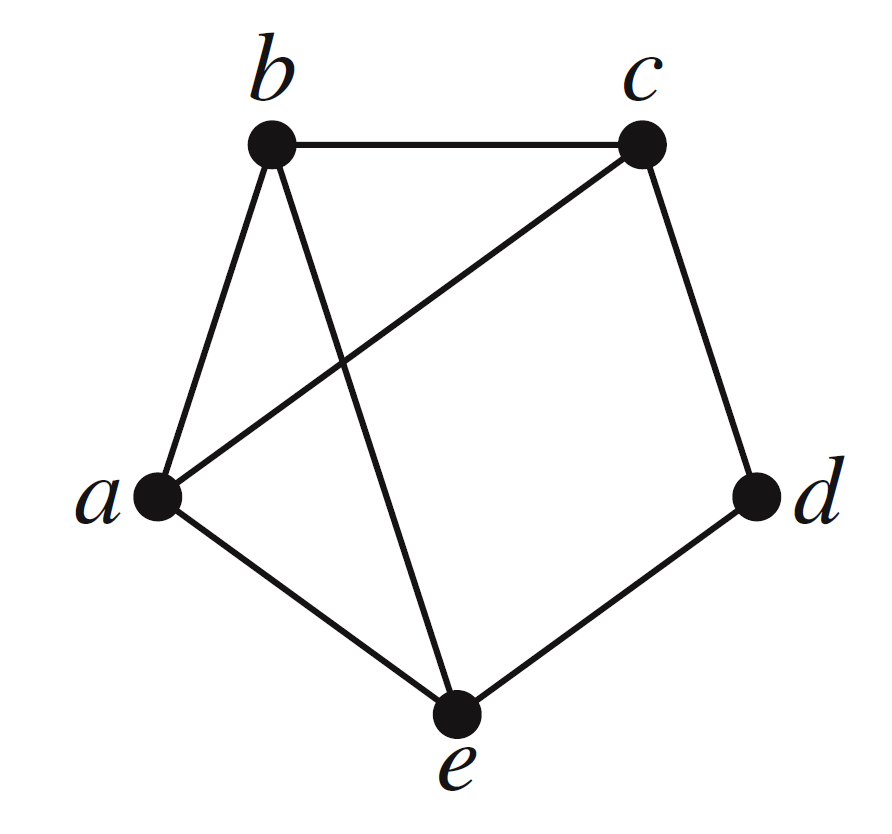
\includegraphics[width=.6\linewidth]{f-10-5-e-1}
            \end{figure}
        \end{column}
    \end{columns}
    \onslide<2>\begin{solution*}
        Neither.
    \end{solution*}
\end{frame}

\begin{frame}[fragile]
    \frametitle{Euler Circuit}
    \onslide<1->\begin{columns}
        \begin{column}{.5\linewidth}
            \begin{eg}
                Determine whether the given graph has an
                Euler circuit. Construct such a circuit when one exists. If
                no Euler circuit exists, determine whether the graph has an
                Euler path and construct such a path if one exists.
            \end{eg}
        \end{column}
        \begin{column}{.5\linewidth}
            \begin{figure}
                \centering
                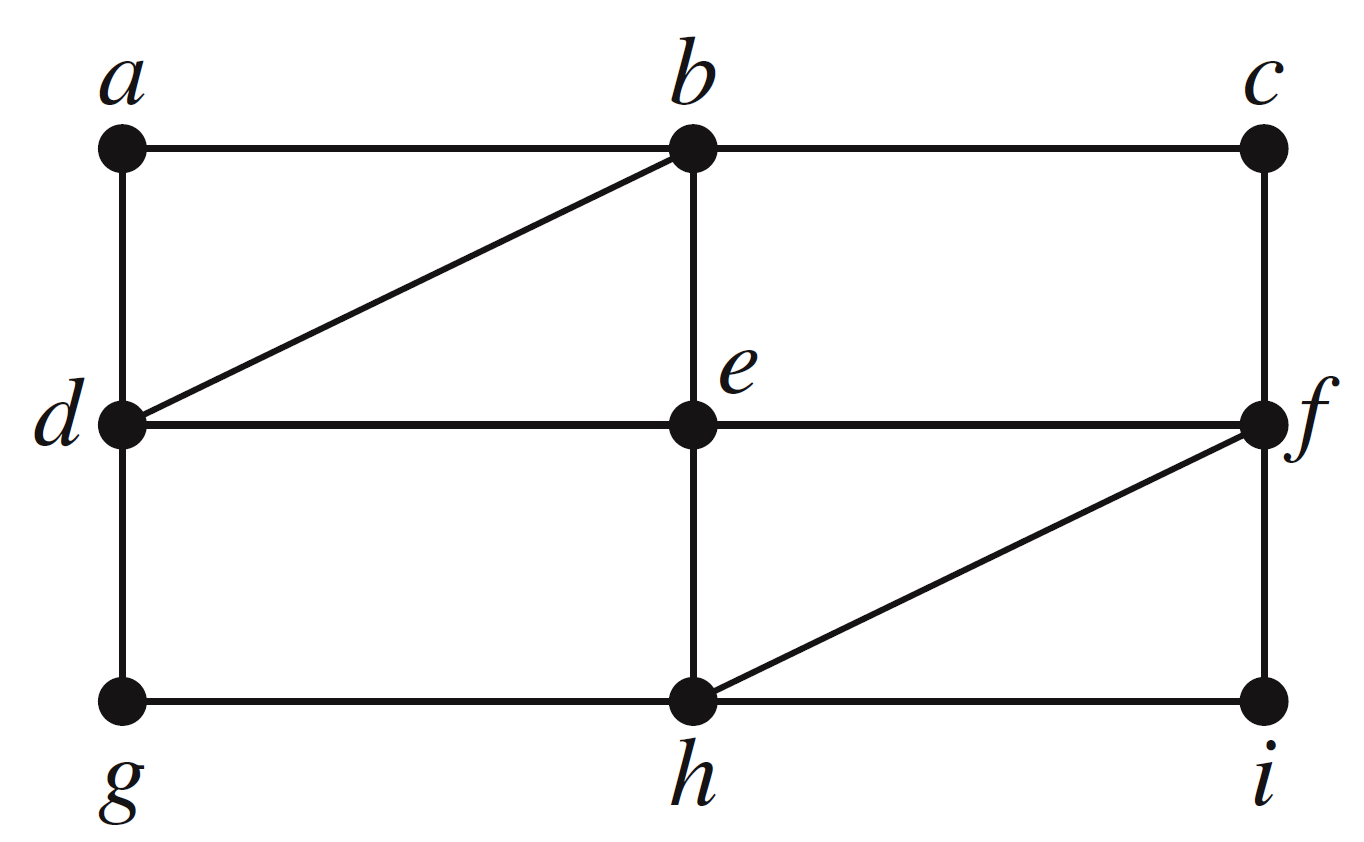
\includegraphics[width=.8\linewidth]{f-10-5-e-2}
            \end{figure}
        \end{column}
    \end{columns}
    \onslide<2>\begin{solution*}
        $a, b, c, f, e, b, d, e, h, f, i, h, g, d, a.$
    \end{solution*}
\end{frame}

\begin{frame}[fragile]
    \frametitle{Hamilton Path}
    \onslide<1->\begin{columns}
        \begin{column}{.5\linewidth}
            \begin{eg}
                Which of the simple graphs in Figure have a Hamilton circuit or, if not, a Hamilton path?
            \end{eg}
        \end{column}
        \begin{column}{.5\linewidth}
            \begin{figure}
                \centering
                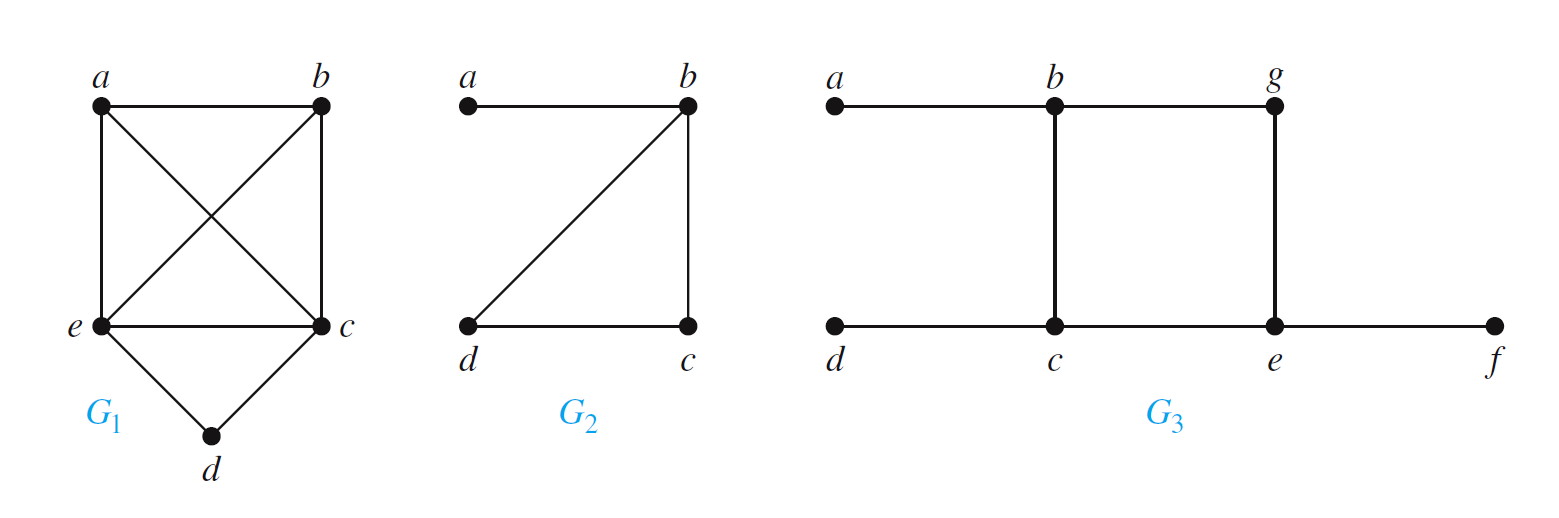
\includegraphics[width=\linewidth]{f-10-5-10}
            \end{figure}
        \end{column}
    \end{columns}
    \onslide<2>\begin{solution*}
        $G_1$ has a Hamilton circuit: $a, b, c, d, e, a$. There is no Hamilton circuit in $G_2$ (this can
        be seen by noting that any circuit containing every vertex must contain the edge $\{a, b\}$ twice),
        but $G_2$ does have a Hamilton path, namely, $a, b, c, d$. $G_3$ has neither a Hamilton circuit nor a
        Hamilton path, because any path containing all vertices must contain one of the edges $\{a, b\}, \{e, f\}$, and $\{c, d\}$ more than once.
    \end{solution*}
\end{frame}

\begin{frame}[fragile]
    \frametitle{Hamilton Circuit}
    \onslide<1->\begin{columns}
        \begin{column}{.5\linewidth}
            \begin{eg}
                Show that neither graph displayed in Figure has a Hamilton circuit.
            \end{eg}
        \end{column}
        \begin{column}{.5\linewidth}
            \begin{figure}
                \centering
                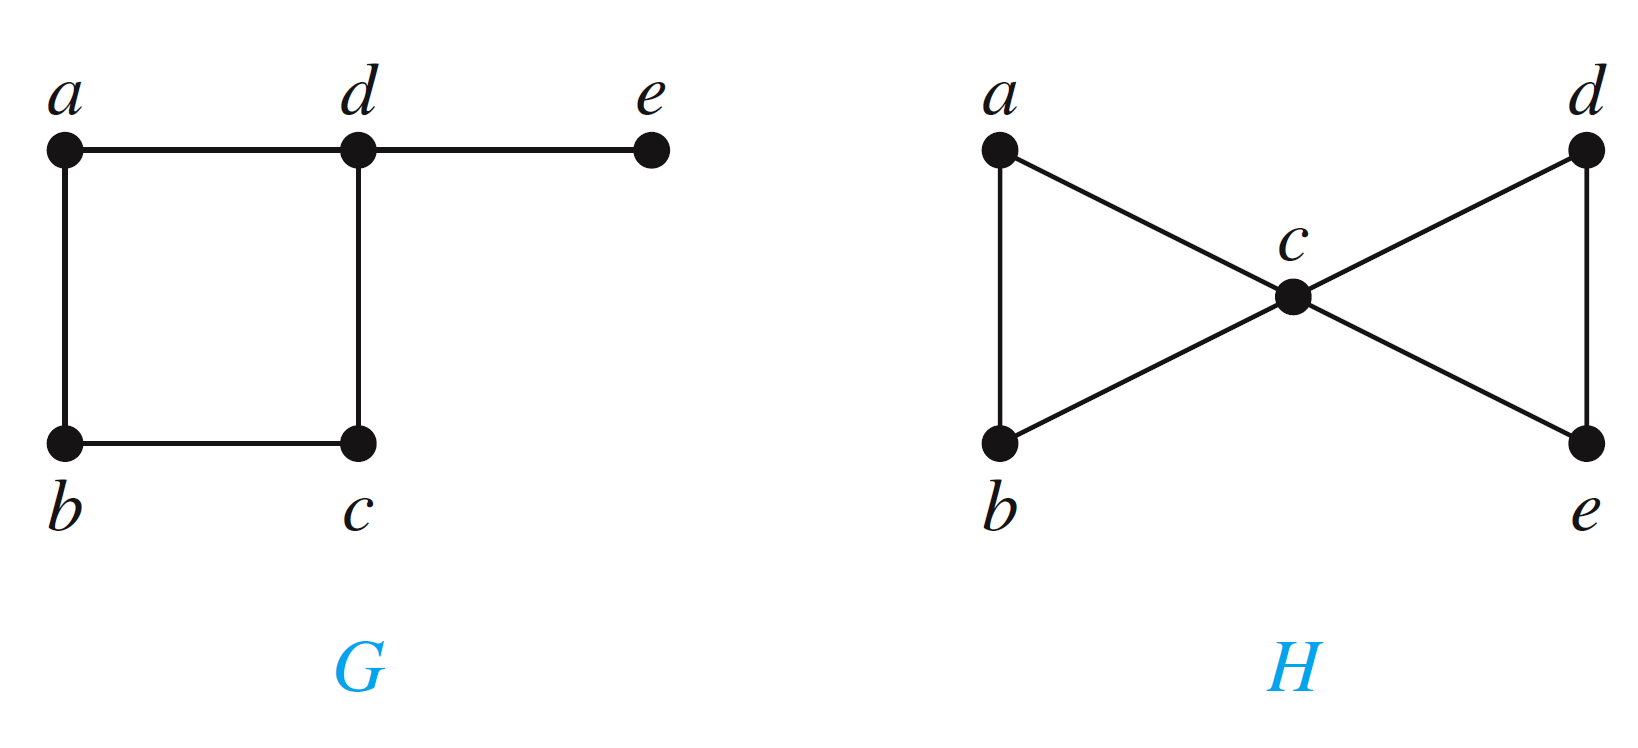
\includegraphics[width=\linewidth]{f-10-5-11}
            \end{figure}
        \end{column}
    \end{columns}
    \onslide<2>\begin{solution*}
        There is no Hamilton circuit in $G$ because $G$ has a vertex of degree one, namely, $e$. Now consider $H$. Because the degrees of the vertices $a, b, d$, and $e$ are all two, every edge incident with these vertices must be part of any Hamilton circuit. It is now easy to see that no Hamilton circuit can exist in $H$, for any Hamilton circuit would have to contain four edges incident with c, which is impossible.
    \end{solution*}
\end{frame}

\subsection{Shortest-Path Problems}

\begin{frame}[fragile]
    \frametitle{Shortest Path}
    \onslide<1->\begin{columns}
        \begin{column}{.5\linewidth}
            \begin{eg}
                Find the length of a shortest path between $a$
                and $z$ in the given weighted graph.
            \end{eg}
        \end{column}
        \begin{column}{.5\linewidth}
            \begin{figure}
                \centering
                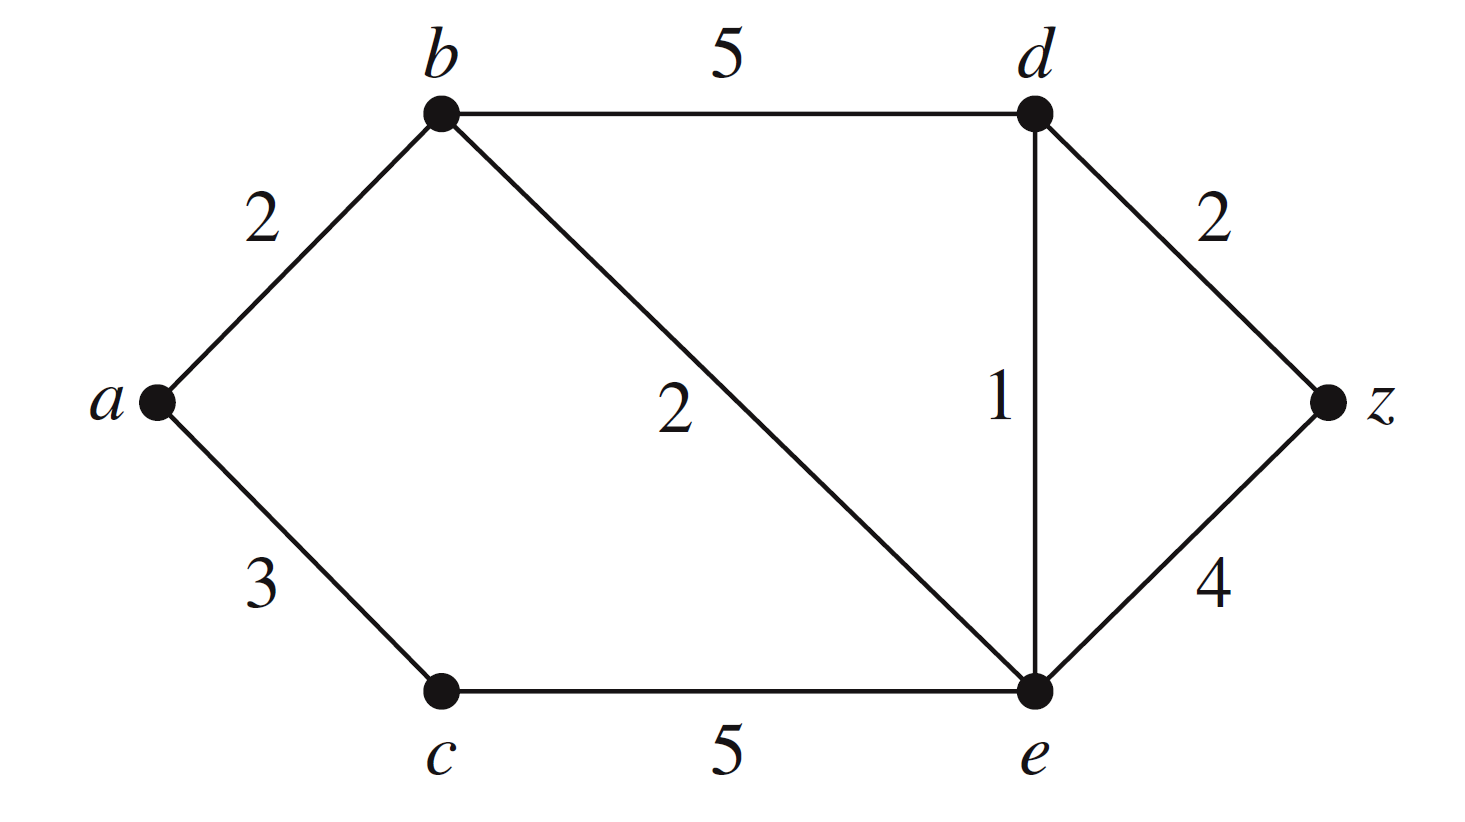
\includegraphics[width=\linewidth]{f-10-6-e-2}
            \end{figure}
        \end{column}
    \end{columns}
    \onslide<2>\begin{solution*}
        \begin{equation}
        2 + 2 + 1 + 2 = 7.
        \end{equation}
    \end{solution*}
\end{frame}

\section{Trees}
\subsection{Introduction to Trees}

\begin{frame}[fragile]
    \frametitle{Tree}
    \begin{theorem}
        An undirected graph is a tree if and only if there is a unique path without cycle between any two of its vertices.
    \end{theorem}
    \onslide<2>\begin{proof}
        First assume that $T$ is a tree which is connected graph without cycle.
        Because $T$ is connected, there is a path without cycle between two vertices $x$ and $y$.
        Moreover, this path must be unique, for if there were a second such path,
        they would form a cycle.    
        This implies that there is a cycle in $T$.
        
        Now assume that there is a unique path without cycle between any two vertices of a graph $T$.
        Then $T$ is connected, because there is a path between any two of its vertices.
        Furthermore, $T$ can have no cycles.
        To see that this is true, suppose $T$ had a cycle that contained the vertices $x$ and $y$.
        Then there would be two simple paths between $x$ and $y$.
    \end{proof}
\end{frame}

\begin{frame}[fragile]
    \frametitle{Left Child}
    \begin{columns}
        \begin{column}{.6\linewidth}
            \onslide<1->\begin{eg}
                What are the left and right children of $d$ in the binary tree $T$ shown in Figure \ref{f-11-1-8} (where the order is that implied by the drawing)? What are the left and right subtrees of $c$?
            \end{eg}
            \onslide<2>\begin{solution*}
                The left child of $d$ is $f$ and the right child is $g$.
            \end{solution*}
        \end{column}
        \onslide<1->\begin{column}{.4\linewidth}
            \begin{figure}
                \centering
                $\Tree [.a [.b [.d f g ] e ] [.c [.h j ] [.i k [.l m ]]]]$
                \caption{A Binary Tree $T$}
                \label{f-11-1-8}
            \end{figure}
        \end{column}
    \end{columns}
\end{frame}

\begin{frame}[fragile]
    \frametitle{$m$-ary Tree}
    \onslide<1->\begin{theorem}\label{t-11-1-3}
        A full $m$-ary tree with $i$ internal vertices contains $n = m i + 1$ vertices.
    \end{theorem}
    \onslide<2>\begin{proof}
        Every vertex, except the root, is the child of an internal vertex. Because each of the $i$ internal vertices has $m$ children, there are $m i$ vertices in the tree other than the root. Therefore, the tree contains $n = m i + 1$ vertices
    \end{proof}
\end{frame}

\subsection{Applications of Trees}

\begin{frame}
    \frametitle{Sorting Algorithm}
    \begin{theorem} \label{t-11-2-1}
        A sorting algorithm based on binary comparisons requires at least $\lceil \log n! \rceil$ comparisons.
    \end{theorem}
    \onslide<2>\begin{proof}
        The complexity of a sort based on binary comparisons
        is measured in terms of the number of such comparisons used.
        The largest number of binary comparisons ever needed to sort a list with $n$ elements gives the worst-case performance of the algorithm. The most comparisons used equals the longest path length in the decision tree representing the sorting procedure. In other words, the largest number of comparisons ever needed is equal to the height of the decision tree.
        Because the height of a binary tree with $n!$ leaves is at least $\lceil \log n! \rceil$, at least $\lceil \log n! \rceil$ comparisons are needed.
    \end{proof}
\end{frame}

\plain{Questions?}

\end{document}
